%%%%%%%%%%%%%%%%%%%%%%%%%%%%%%%%%%%%%%%%%
% Short Sectioned Assignment
% LaTeX Template
% Version 1.0 (5/5/12)
%
% This template has been downloaded from:
% http://www.LaTeXTemplates.com
%
% Original author:
% Frits Wenneker (http://www.howtotex.com)
%
% License:
% CC BY-NC-SA 3.0 (http://creativecommons.org/licenses/by-nc-sa/3.0/)
%
%%%%%%%%%%%%%%%%%%%%%%%%%%%%%%%%%%%%%%%%%

%----------------------------------------------------------------------------------------
%	PACKAGES AND OTHER DOCUMENT CONFIGURATIONS
%----------------------------------------------------------------------------------------

\documentclass[paper=a4, fontsize=11pt]{article} % A4 paper and 11pt font size

\usepackage[T1]{fontenc} % Use 8-bit encoding that has 256 glyphs
% \usepackage{fourier} % Use the Adobe Utopia font for the document - comment this line to return to the LaTeX default
\usepackage[english]{babel} % English language/hyphenation
\usepackage{amsmath,amsfonts,amsthm} % Math packages
\usepackage{geometry}
\geometry{left=2.5cm, right=2.5cm, top=2.5cm, bottom=2.5cm}
% \usepackage{lipsum} % Used for inserting dummy 'Lorem ipsum' text into the template

% \usepackage{sectsty} % Allows customizing section commands
\usepackage{graphicx}
\graphicspath{ {C:/Users/Charles/github/ifnet/figures/mi_estimation/} }
\usepackage{float}
\usepackage{multirow}
% \allsectionsfont{\centering \normalfont\scshape} % Make all sections centered, the default font and small caps

\usepackage{fancyhdr} % Custom headers and footers
\pagestyle{fancyplain} % Makes all pages in the document conform to the custom headers and footers
\fancyhead{} % No page header - if you want one, create it in the same way as the footers below
\fancyfoot[L]{} % Empty left footer
\fancyfoot[C]{} % Empty center footer
\fancyfoot[R]{\thepage} % Page numbering for right footer
\renewcommand{\headrulewidth}{0pt} % Remove header underlines
\renewcommand{\footrulewidth}{0pt} % Remove footer underlines
\setlength{\headheight}{13.6pt} % Customize the height of the header

\numberwithin{equation}{section} % Number equations within sections (i.e. 1.1, 1.2, 2.1, 2.2 instead of 1, 2, 3, 4)
\numberwithin{figure}{section} % Number figures within sections (i.e. 1.1, 1.2, 2.1, 2.2 instead of 1, 2, 3, 4)
\numberwithin{table}{section} % Number tables within sections (i.e. 1.1, 1.2, 2.1, 2.2 instead of 1, 2, 3, 4)

\setlength\parindent{0pt} % Removes all indentation from paragraphs - comment this line for an assignment with lots of text

%----------------------------------------------------------------------------------------
%	TITLE SECTION
%----------------------------------------------------------------------------------------

\newcommand{\horrule}[1]{\rule{\linewidth}{#1}} % Create horizontal rule command with 1 argument of height

\title{
\normalfont \normalsize
% \textsc{university, school or department name} \\ [25pt] % Your university, school and/or department name(s)
\horrule{0.5pt} \\[0.4cm] % Thin top horizontal rule
\huge Deduce: Deviation of mutual information estimation \\ % The assignment title
\horrule{2pt} \\[0.5cm] % Thick bottom horizontal rule
}

% \author{John Smith} % Your name

\date{\normalsize\today} % Today's date or a custom date

\begin{document}

\maketitle % Print the title

%----------------------------------------------------------------------------------------
%	PROBLEM 1
%----------------------------------------------------------------------------------------

% \section{Problem title}

% \lipsum[2] % Dummy text

\begin{align}
\begin{split}
I_{true}(X;Y) &= \int_y \int_x F(x,y)log\frac{F(x,y)}{f(x)g(y)}dxdy\\
&=\sum_{y_i}\sum_{x_i}\int_{y_i}^{y_i + \triangle y} \int_{x_i}^{x_i + \triangle x} F(x,y)log\frac{F(x,y)}{f(x)g(y)}dxdy\\
&=\sum_{y_i}\sum_{x_i} F(x_i^c,y_i^c)log\frac{F(x_i^c,y_i^c)}{f(x_i^c)g(y_i^c)}\triangle x \triangle y
\end{split}
\end{align}

\begin{equation}
  I_{obs}(X;Y) 	= \sum_y \sum_x P(x,y)log\frac{P(x,y)}{P(x)P(y)}
\end{equation}

\begin{align}
\begin{split}
P(x_i,y_j) &= \int\limits_{\triangle y} \int\limits_{\triangle x} F(x_i,y_j)dx_idy_j = F(\hat{x}_i, \hat{y}_j)\triangle x \triangle y
\end{split}
\end{align}
Similarly,
\begin{align}
\begin{split}
&P(x_i) = f(\tilde{x}_i)\triangle x\\
&P(y_j) = g(\tilde{y}_j)\triangle y
\end{split}
\end{align}
Here, take Taylor expension of $F(x_i^c,y_j^c)$, $f(x_i^c)$, $g(y_j^c)$ around (x,y) = $(\hat{x}_i, \hat{y}_j)$, x = $\tilde{x}_i$, y = $\tilde{y}_j$, respectively.
\begin{align}
	\begin{split}
		F(x_i^c, y_j^c) &= F(\hat{x}_i, \hat{y}_j) + \frac{\partial F}{\partial x}(x_i^c-\hat{x}_i) + \frac{\partial F}{\partial y}(y_j^c-\hat{y}_j) +  \frac{1}{2}\frac{\partial^2 F}{\partial x\partial y}(x_i^c-\hat{x}_i)(y_j^c-\hat{y}_j) + ... \\
		f(x_i^c) &= f(\tilde{x}_i) + \frac{df}{dx}(x_i^c-\tilde{x}_i) + \frac{1}{2}\frac{d^2f}{dy}(x_i^c-\tilde{x}_i)^2 + ...\\
		g(y_j^c) &= g(\tilde{y}_j) + \frac{dg}{dy}(y_j^c-\tilde{y}_j) + \frac{1}{2}\frac{d^2g}{dy}(y_j^c-\tilde{y}_j)^2 + ...
	\end{split}
\end{align}

Since $|x_i^c - \hat{x}_i| <= \triangle x$, $|y_j^c - \hat{y}_j| <= \triangle y$, $\triangle x = \triangle y = h$,

\begin{align}
	\begin{split}
		F(x_i^c, y_j^c) &= F(\hat{x}_i, \hat{y}_j) + (\frac{\partial F}{\partial x}\hat{c}_i + \frac{\partial F}{\partial y}\hat{c}_j)h + O(h^2)\\
		f(x_i^c) &= f(\tilde{x}_i) + \frac{df}{dx}\tilde{c}_ih + O(h^2)\\
		g(y_j^c) &= g(\tilde{y}_j) + \frac{dg}{dy}\tilde{c}_jh + O(h^2)
	\end{split}
\end{align}

Substitute those expression into the expression of mutual information.

\begin{align}
\begin{split}
	I_{true}(X;Y) &\doteq\sum_{y_i}\sum_{x_i} F(x_i^c,y_i^c)\triangle x \triangle y[log(F(x_i^c,y_i^c)\triangle x\triangle y)-log(f(x_i^c)\triangle x) - log(g(y_i^c)\triangle y)]\\
	&= \sum_{y_i}\sum_{x_i} [P(x_i, y_j) + (\frac{\partial F}{\partial x}\hat{c}_i + \frac{\partial F}{\partial y}\hat{c}_j)h^3] \\
	&[log(P(x_i, y_j) + (\frac{\partial F}{\partial x}\hat{c}_i + \frac{\partial F}{\partial y}\hat{c}_j)h^3) - log(P(x_i) + \frac{df}{dx}\tilde{c}_ih^2) - log(P(y_j) + \frac{dg}{dy}\tilde{c}_jh^2))]
\end{split}
\end{align}

Take Taylor expansion of logarithmic function to the first order,

\begin{align}
\begin{split}
	I_{true}(X;Y)	&\doteq \sum_{y_i}\sum_{x_i} (P(x_i, y_j) + (\frac{\partial F}{\partial x}\hat{c}_i + \frac{\partial F}{\partial y}\hat{c}_j)h^3) \\
	&(logP(x_i, y_j) + (\frac{\partial F}{\partial x}\hat{c}_i + \frac{\partial F}{\partial y}\hat{c}_j)h^3 - logP(x_i) - \frac{df}{dx}\tilde{c}_ih^2 - logP(y_j) - \frac{dg}{dy}\tilde{c}_jh^2) \\
	&= \sum_{y_i}\sum_{x_i} (P(x_i, y_j) + (\frac{\partial F}{\partial x}\hat{c}_i + \frac{\partial F}{\partial y}\hat{c}_j)h^3) \\
	&(log\frac{P(x_i, y_j)}{P(x_i)P(y_j)} + (\frac{\partial F}{\partial x}\hat{c}_i + \frac{\partial F}{\partial y}\hat{c}_j)h^3 - (\frac{df}{dx}\tilde{c}_i + \frac{dg}{dy}\tilde{c}_j)h^2)
\end{split}
\end{align}

Drop higher order terms which is sufficiently smaller than $O(h^2)$.

\begin{align}
\begin{split}
	I_{true}(X;Y)	&\doteq \sum_{y_j}\sum_{x_i} P(x_i, y_j) (logP(x_i, y_j) - logP(x_i) - \frac{df}{dx}\tilde{c}_ih^2 - logP(y_j) - \frac{dg}{dy}\tilde{c}_jh^2) \\
	&= \sum_{y_j}\sum_{x_i}P(x_i, y_j)(log\frac{P(x_i, y_j)}{P(x_i)P(y_j)} - (\frac{df}{dx}\tilde{c}_i + \frac{dg}{dy}\tilde{c}_j)h^2) \\
	&= I_{obs} - \sum_{y_j}\sum_{x_i}P(x_i,y_j)(\frac{df}{dx}\tilde{c}_i + \frac{dg}{dy}\tilde{c}_j)h^2
\end{split}
\end{align}

Since $\tilde{c}_i$ and $\tilde{c}_j$ are constants, they can obsorbe the negative sign outside the summation. Therefore, the deviation of mutual information estimation with finite, equally binned histogram from its true value given by the expression below:

\begin{align}
	\begin{split}
		I_{true}	- I_{obs} = h^2\sum_{y_j}\sum_{x_i}P(x_i,y_j)(\frac{df}{dx}\tilde{c}_i + \frac{dg}{dy}\tilde{c}_j) + O(h^3)
	\end{split}
	\label{equ:gauss_mi}
\end{align}

In the next part, numerical results are presented to varify the analytical results above.

$X$ and $Y$ are two random variables generated by the following equations.

$$\left\{
\begin{aligned}
	\begin{split}
		X &= \epsilon \\
		Y &= \beta\eta_1 + \xi X + \eta_2
	\end{split}
\end{aligned}
\right.$$

where $\epsilon$ and $\eta_i$ are independent normally distributed random variables, and $\beta$ and $\xi$ are interacting strength between variables. Here, $X$ and $Y$ both contain $10^8$ independent samples. We calculate the mutual information between $X$ and $Y$ using theoretical expression and numerical estimation, respectively. And we can get the deviation of mutual information estimation from its true value, which given by theoretical expression, as a function of binning size.

\begin{figure}[H]
	\centering
	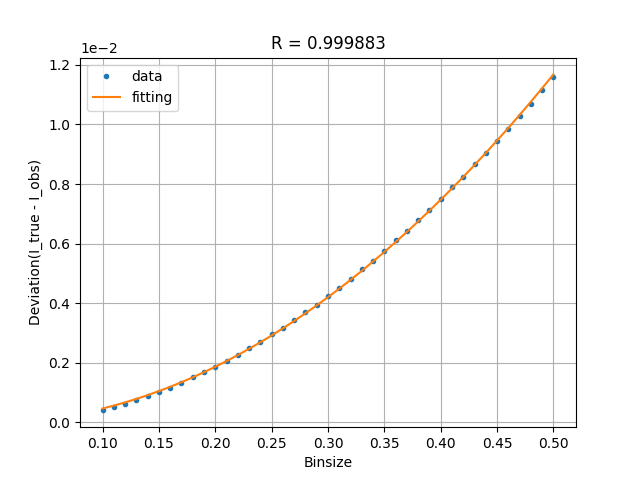
\includegraphics[scale = 0.7]{gauss_mi_max_1e8.png}
	\caption{Accuracy of mutual information estimation as a function of bin size of histograms of variables.}
	\label{fig:gauss_mi_max}
\end{figure}

We find that the data points are nicely fitted by second order polynormial given by $y= ax^2$. This result verify our deduction above.

Then we move the case for mutual information between binary spike train $X$ and continues neuronal data $Y$, which is net synaptic current of single neuron. We demonstrate a two excitatory neuron system simulated with conductance-based leaky integrate-and-fire model. Two neuron, which labeled as neuron-1 and neuron-2 respectively, are one-way connected, meaning neuron-1 can transmit its spike train to neuron-2 but not counterwise. We record spike train from neuron-1 as $X$ and synaptic current from neuron-2 as $Y$. The simulating parameters of this system are listed below.

\begin{table}[H]
	\centering
	\begin{tabular}{c|c}
		\hline
		\hline
		Total time period & $10^8$ ms \\
		Recording rate & 2 $ms^-1$ \\
		Synaptic strength & $5^-2$ \\
		Poisson rate & 1.3 kHz \\
		Poisson strength & $5^{-2}$ \\
		\hline
		\hline
	\end{tabular}
\end{table}

Since $X$ is a binary variable, the expression in \ref{equ:gauss_mi} needs to be modified.

\begin{align}
	\begin{split}
		I_{true}	- I_{obs} &= h^2\left[\sum_{y_i}\left.\frac{\partial F}{\partial y}\right|_{x=0}c_ilog\frac{P(x=0,y_i)}{P(x=0)P(y_i)} + \left.\frac{\partial F}{\partial y}\right|_{x=1}c_i'log\frac{P(x=1,y_i)}{P(x=1)P(y_i)}\right. \\
		&\left.+ P(x=0,y_i)(\left.\frac{\partial F}{\partial y}\right|_{x=0}c_i- \frac{dg}{dy}\hat{c}_i + P(x=1,y_i)(\left.\frac{\partial F}{\partial y}\right|_{x=1}c_i') - \frac{dg}{dy}\hat{c}_i')\right] + o(h^2)
	\end{split}
\end{align}

\begin{figure}[H]
	\centering
	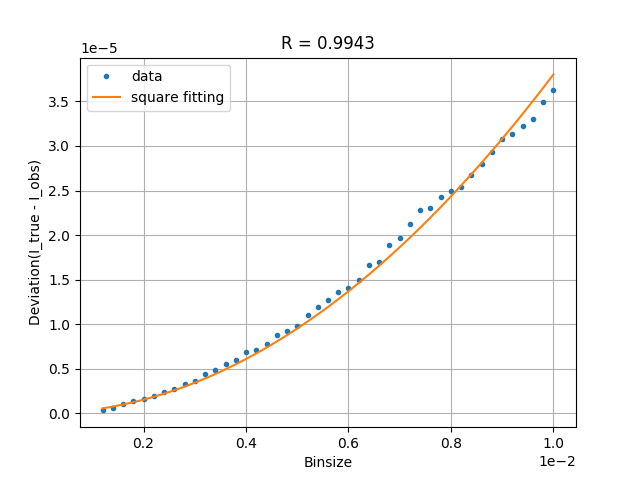
\includegraphics[scale = 0.7]{mi_bd_max_dx_1e8.png}
	\caption{Accuracy of mutual information estimation as a function of bin size of histograms of variables.}
	\label{fig:mi_max}
\end{figure}

The orange line is the linear fitting given by $y = ax$ and the green curve is the square fitting given by $y = ax^2$.

%------------------------------------------------

% \subsection{Heading on level 2 (subsection)}
%
% Lorem ipsum dolor sit amet, consectetuer adipiscing elit.
% \begin{align}
% A =
% \begin{bmatrix}
% A_{11} & A_{21} \\
% A_{21} & A_{22}
% \end{bmatrix}
% \end{align}
% Aenean commodo ligula eget dolor. Aenean massa. Cum sociis natoque penatibus et magnis dis parturient montes, nascetur ridiculus mus. Donec quam felis, ultricies nec, pellentesque eu, pretium quis, sem.
%
% %------------------------------------------------
%
% \subsubsection{Heading on level 3 (subsubsection)}
%
% % \lipsum[3] % Dummy text
%
% \paragraph{Heading on level 4 (paragraph)}
%
% % \lipsum[6] % Dummy text
%
% %----------------------------------------------------------------------------------------
% %	PROBLEM 2
% %----------------------------------------------------------------------------------------
%
% \section{Lists}
%
% %------------------------------------------------
%
% \subsection{Example of list (3*itemize)}
% \begin{itemize}
% 	\item First item in a list
% 		\begin{itemize}
% 		\item First item in a list
% 			\begin{itemize}
% 			\item First item in a list
% 			\item Second item in a list
% 			\end{itemize}
% 		\item Second item in a list
% 		\end{itemize}
% 	\item Second item in a list
% \end{itemize}
%
% %------------------------------------------------
%
% \subsection{Example of list (enumerate)}
% \begin{enumerate}
% \item First item in a list
% \item Second item in a list
% \item Third item in a list
% \end{enumerate}

%----------------------------------------------------------------------------------------

\end{document}
